\documentclass[dvipdfmx]{jsarticle}
\usepackage[dvipdfmx]{graphicx}
\usepackage{here}


\begin{document}
\section*{2.5 多層パーセプトロン}
本節では,多層パーセプトロンと,層を重ねることによるXORの実現について説明されている.
ただし,「層を重ねる」ことの詳細については本節では記述されていない.

\section*{2.5.1 既存ゲートの組み合わせ}
XORゲートを作るにはいくつかの方法がある.一つの方法は,既出のAND,NAND,ORゲートを組み合わせて配線することである.図1に各ゲートの記号を示す.なお,NANDゲートの先端の○は出力の反転を意味する.


\begin{figure}[htbp]
    \begin{center}
        
\includegraphics[width=\linewidth]{spring_lec/dp_gate.png}
    \end{center}
    \caption{AND,NAND,ORゲートの記号}
\end{figure}

図1を参考に,図2の「?」のそれぞれにANDとNANDとORをうまく配線すると,XORを完成させることができる.

\begin{figure}[htbp]
\begin{center}

\includegraphics[width=\linewidth]{spring_lec/dp_xor.png}
\end{center}
\caption{AND,NAND,ORゲートのいずれかを「?」に挿入してXORを完成させよう!}
\end{figure}

\begin{figure}[htbp]
\begin{center}

\includegraphics[width=\linewidth]{spring_lec/dp_xor2.png}
\end{center}
\caption{AND,NAND,ORゲートの組み合わせによってXORゲートを実現する}
\end{figure}

\newpage
XORゲートは図3の配線で実現できる.ここでは,$x_1$と$x_2$が入力信号,$y$が出力信号を表している.$x_1$と$x_2$はNANDとORゲートへの入力であり,NANDとORの出力がANDゲートの入力となっている.

ここで,図3の配線が正しくXORを実現できているかを確かめる.図の真理値表は,NANDの出力を$s_1$,ORの出力を$s_2$としている.真理値表から,確かにXORの出力となっていることが分かる.

\begin{figure}[htbp]
\begin{center}
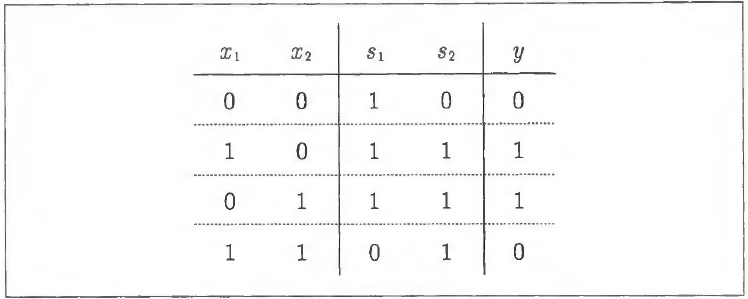
\includegraphics[width=\linewidth]{spring_lec/dp_xor_chart.png}
\end{center}
\caption{XORゲートの真理値表}
\end{figure}

こうして実現したXORゲートをパーセプトロンによって表記すると,図5のようになる.
XORは,図のような多層構造のネットワークとなり,既出のANDやORといった単層のパーセプトロンとは異なる形をしている.XORは,合計で3層から構成されるが,重みを持つ層は実質2層であるため,2層のパーセプトロンである(3層のパーセプトロンと呼ぶ場合もある).

このように,層を複数重ねたパーセプトロンを\textbf{多層パーセプトロン}(multi-layered perceptron)と呼ぶ.
前節で述べられたパーセプトロンの限界とは,正確に言えば,「単層のパーセプトロンではXORゲートを表現できない」または「単層のパーセプトロンでは非線形領域は分離できない」ということであったが,多層パーセプトロンを用いることで,その限界に縛られない表現が可能になる.

\begin{figure}[H]
\begin{center}
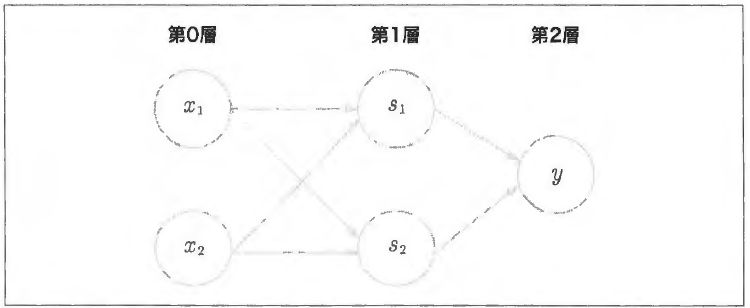
\includegraphics[width=\linewidth]{spring_lec/dp_multi.png}
\end{center}
\caption{XORのパーセプトロンによる表記}
\end{figure}

\end{document}]